\documentclass[a4paper]{article}

\usepackage{a4wide}
\usepackage{amsmath}
\usepackage{amssymb}
\usepackage{amsthm}
\usepackage{enumitem}
    \setlist[enumerate]{label=(\alph*),itemsep=3pt,topsep=6pt}
    \setlist[itemize]{itemsep=3pt,topsep=6pt}
\usepackage{tikz}
\usepackage[utf8]{inputenc}


\theoremstyle{definition}
\newtheorem{problem}{Příklad}
\newtheorem*{ukol}{Domácí úkol}


\begin{document}

\section*{NAIL062 V\&P Logika: 13. cvičení}


\textbf{Témata:}
(Zápočtový test z predikátové logiky.) Vybraná témata z teorie modelů.


\medskip\begin{problem}
    Buď $T=\{(\forall x)(\exists y) S(y)=x,\ S(x)=S(y)\to x=y\}$ teorie v~jazyce $L=\langle S\rangle$ s~rovností, kde $S$ je unární funkční symbol.
    \begin{enumerate}
    \item Buď $\mathcal{R}=\langle\mathbb{R},S\rangle$, kde $S(r)=r+1$ pro $r\in\mathbb{R}$. Právě pro která $r\in\mathbb{R}$ je množina $\{r\}$ definovatelná v~$\mathcal{R}$ z~parametru $0$?
    \item Je teorie $T$ otevřeně axiomatizovatelná? Uveďte zdůvodnění.
    \item Je extenze $T'$ teorie $T$ o~axiom $S(x)=x$ $\omega$-kategorická teorie? Je $T'$ kompletní?
    \item Pro která $0<n\in\mathbb{N}$ existuje $L$-struktura $\mathcal{B}$ velikosti $n$ elementárně ekvivalentní s~$\mathcal{R}$? Existuje spočetná struktura $\mathcal{B}$ elementárně ekvivaletní s~$\mathcal{R}$?
    \end{enumerate}
\end{problem}


\medskip\begin{problem}
Uvažme následující graf:
\begin{center}
    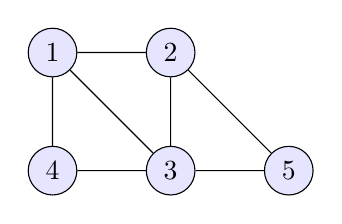
\begin{tikzpicture}[every node/.style={circle,fill=blue!10,draw,minimum size=0.5cm,node distance=1.5cm}]
        \node (1) {$1$};
        \node[right of=1] (2) {$2$};
        \node[below of=2] (3) {$3$};
        \node[left of=3] (4) {$4$};
        \path[draw] (1) -- (2) -- (3) -- (4) -- (1) -- (3);
        \node[right of=3] (5) {$5$};
        \path[draw] (2) -- (5) -- (3);
    \end{tikzpicture}
\end{center}
\begin{enumerate}
    \item Najděte všechny automorfismy.
    \item Které podmnožiny množiny vrcholů $V$ jsou definovatelné? Uveďte definující formule. {\it (Nápověda: Využijte (a).)}
    \item Které binární relace na $V$ jsou definovatelné?
\end{enumerate}
\end{problem}



\medskip\begin{problem}
    Nechť $T = \{U(x) \to U(f(x)), (\exists x)U(x), \neg (f(x) = x), \varphi\}$ je teorie v jazyce $L = \langle U, f \rangle$ s rovností, kde $U$ je unární relační symbol, $f$ je unární funkční symbol a $\varphi$ vyjadřuje, že ``existují maximálně 4 prvky''.
    \begin{enumerate}
    \item Je teorie $T$ extenzí teorie $S = \{ (\exists x)(\exists y)(\neg x = y \land U(x) \land U(y)), \varphi \}$ v jazyce $L' = \langle U \rangle$? Je konzervativní extenzí? Zdůvodněte.
    \item Je teorie $T$ otevřeně axiomatizovatelná? Zdůvodněte.
    \end{enumerate} 
\end{problem}

\medskip\begin{problem}
Nechť $T=\{\varphi\}$ je teorie jazyka $L=\langle U, c \rangle$ s rovností, kde $U$ je unární relační symbol, $c$ je konstantní symbol a axiom $\varphi$ vyjadřuje \emph{``Existuje alespoň $5$ prvků, pro které platí U(x).''}
\begin{enumerate}
\item Nalezněte dvě neekvivalentní jednoduché kompletní extenze teorie $T$ nebo zdůvodněte, proč neexistují.
\item Je teorie $T$ otevřeně axiomatizovatelná? Uveďte zdůvodnění.
\end{enumerate}
\end{problem}


\medskip\begin{problem} %move to tutorial 8?
    Buď $T=\{(\forall x)(\exists y) S(y)=x,\ S(x)=S(y)\to x=y\}$ teorie v~jazyce $L=\langle S\rangle$ s~rovností, kde $S$ je unární funkční symbol.
    \begin{enumerate}
    \item Nalezněte extenzi $T'$ teorie $T$ o definici nového unárního funkčního symbolu $P$ takovou, že $T' \models S(S(x))=y \leftrightarrow P(P(y))=x$. {\it (2b)}
    \item Je teorie $T'$ otevřeně axiomatizovatelná? Uveďte zdůvodnění. {\it (2b)}
    \end{enumerate} 
\end{problem} 


\medskip\begin{problem}
    Nechť $T$ je extenze teorie $DeLO^-$ (tj. hustých lineárních uspořádání s minimálním prvkem a bez maximálního prvku) o nový axiom $c \le d$ v jazyce $L=\langle \le,c,d\rangle$ s rovností, kde $c$, $d$ jsou nové konstantní symboly.
    \begin{enumerate}
    \item Jsou sentence $(\exists x)(x\le d \wedge x \ne d)$ a $(\forall x)(x \le d)$ pravdivé / lživé / nezávislé v $T$? Uveďte zdůvodnění.
    \item Napište dvě neekvivalentní jednoduché kompletní extenze teorie $T$.
    \end{enumerate} 
\end{problem}


\medskip\begin{ukol}
Už žádný není. Hodně štěstí u zkoušky (resp. u opravného testu)!
\end{ukol}

\end{document}